\documentclass[logo,reportComp]{thesis}
\usepackage[cpp,pseudo]{mypackage}

\title{数字图像处理作业三}
\subtitle{}
\school{数据科学与计算机学院}
\author{陈鸿峥}
\classname{17大数据与人工智能}
\stunum{17341015}
\headercontext{数字图像处理作业}
\lstset{language=matlab}

\begin{document}

\maketitle
% PROJECT 04-01 - 04-05
本次作业包括PROJECT 04-01到PROJECT 04-05五个实验。

\section{二维快速傅里叶变换(PROJECT 04-01)}
% PROJECT 04-01 [Multiple Uses] Two-Dimensional Fast Fourier Transform
% The purpose of this project is to develop a 2-D FFT program "package" that will be used in several other projects that follow. Your implementation must have the capabilities to: (a) Multiply the input image by (-1)x+y to center the transform for filtering.
% (b) Multiply the resulting (complex) array by a real function (in the sense that the the real coefficients multiply both the real and imaginary parts of the transforms). Recall that multiplication of two images is done on pairs of corresponding elements.
% (c) Compute the inverse Fourier transform. (d) Multiply the result by (-1)x+y and take the real part. (e) Compute the spectrum.
% Basically, this project implements Fig. 4.5. If you are using MATLAB, then your Fourier transform program will not be limited to images whose size are integer powers of 2. If you are implementing the program yourself, then the FFT routine you are using may be limited to integer powers of 2. In this case, you may need to zoom or shrink an image to the proper size by using the program you developed in Project 02-04.
% An approximation: To simplify this and the following projects (with the exception of Project 04-05), you may ignore image padding (Section 4.6.3). Although your results will not be strictly correct, significant simplifications will be gained not only in image sizes, but also in the need for cropping the final result. The principles will not be affected by this approximation.
第一题仅仅是实现一些基本函数,简要说明如下。
\begin{itemize}
    \item [(a)] 由于$\Im[f(x,y)(-1)^{x+y}]=F(u-M/2,v-N/2)$,故将原图乘上$(-1)^{x+y}$后可实现频率域的中心平移
    \item [(b)] 直接乘上常数$c$即可
    \item [(c)] matlab的\verb'ifft2'即可完成逆傅里叶变换
    \item [(d)] 同(a),恢复原图
    \item [(e)] 即复数的模,$|F(u,v)|=\sqrt{R^2(x,y)+I^2(x,y)}$
\end{itemize}

\section{傅里叶谱与平均值(PROJECT 04-02)}
% PROJECT 04-02
% Fourier Spectrum and Average Value (a) Download Fig. 4.18(a) and compute its (centered) Fourier spectrum. (b) Display the spectrum.
% (c) Use your result in (a) to compute the average value of the image.
\subsection{原理}
利用PROJECT 04-01中实现的函数即可求出图片的中心化傅里叶谱,详情请见附录中的代码。

\subsection{实验结果与分析}
傅里叶谱的展示通过了一个伽马变换,虽然噪声较多,但依然能够清晰看出正中间的低频分量。
\begin{figure}[H]
\centering
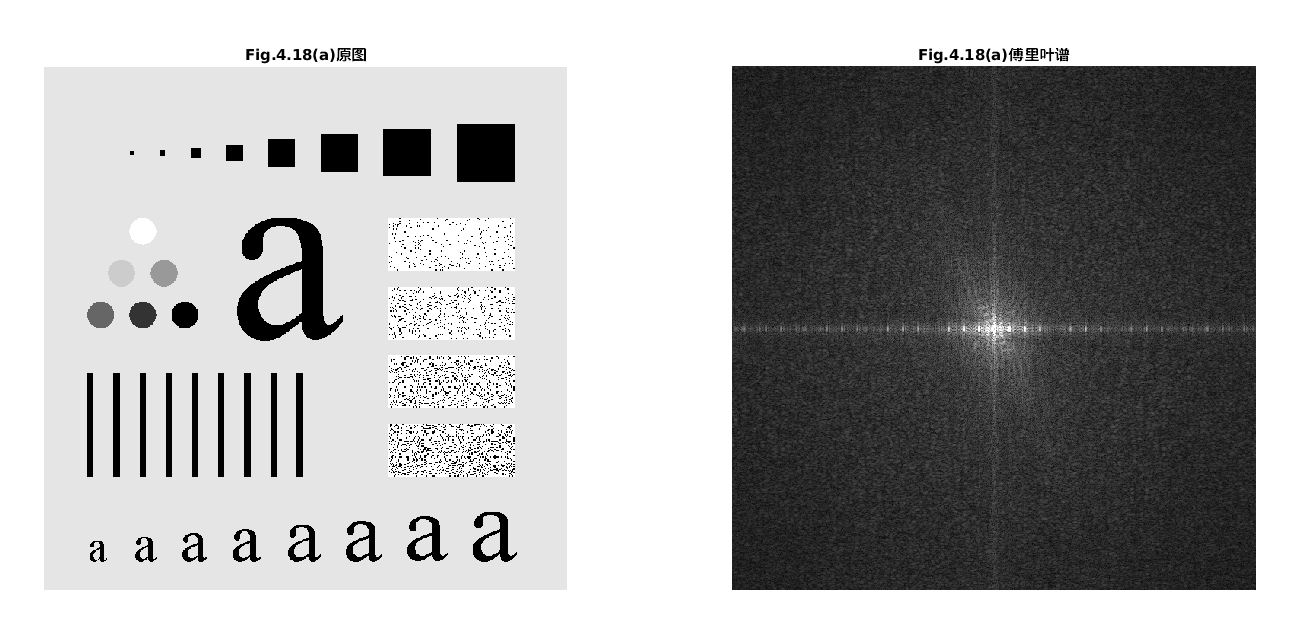
\includegraphics[width=0.8\linewidth]{fig/01.png}
\end{figure}

若在傅里叶变换前没有进行图像中心化,则
\[\frac{1}{MN}F(0,0)=\frac{1}{MN}\sum_{x=0}^{M-1}\sum_{y=0}^{N-1}f(x,y)\]
为图像像素的均值,可求得为$207.31$。

\section{低通滤波器(PROJECT 04-03)}
% PROJECT 04-03 Lowpass Filtering
% (a) Implement the Gaussian lowpass filter in Eq. (4.3-7). You must be able to specify the size, M x N, of the resulting 2D function. In addition, you must be able to specify where the 2D location of the center of the Gaussian function.
% (b) Download Fig. 4.11(a) [this image is the same as Fig. 4.18(a)] and lowpass filter it to obtain Fig. 4.18(c).
\subsection{原理}
二维高斯滤波器由下式给出
\[H(u,v)=\ee^{-D^2(u,v)/2\sigma^2}\]
其中$D(u,v)$为距傅里叶变换原点的距离,$\sigma$为高斯曲线扩展的程度。

频率域滤波的流程如下图所示。
注意这里要进行图像的\textbf{延拓},以确保傅里叶变换的正确性。
\begin{figure}[H]
\centering
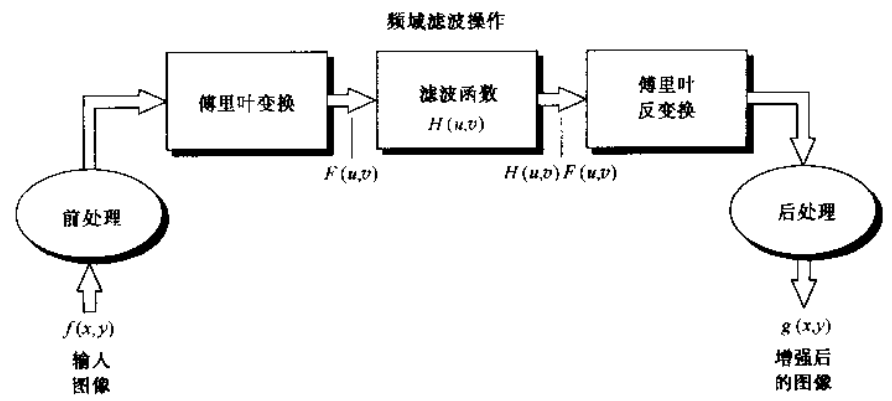
\includegraphics[width=0.8\linewidth]{fig/process.png}
\end{figure}
\begin{enumerate}
	\item 给定大小为$M\times N$的输入图像$f(x,y)$,选择填充参数$P=2M$,$Q=2N$
	\item 对$f(x,y)$添加必要的0,形成大小为$P\times Q$的填充后的图像$f_p(x,y)$
	\item 用$(-1)^{x+y}$乘以$f_p(x,y)$,做频谱中心化处理
	\item 用上面结果计算DFT,得到$F(u,v)$
	\item 生成一个\textbf{实对称}的滤波函数$H(u,v)$,大小为$P\times Q$,中心在$(P/2,Q/2)$处。
	用阵列相乘得到$G(u,v)=H(u,v)F(u,v)$
	\item 计算上式得到的IDFT,并恢复原图像
	\[g_p(x,y)=\Real[\Im[G(u,v)]](-1)^{x+y}\]
	\item 通过从$g_p(x,y)$的左上角提取$M\times N$大小的区域,得到最终结果$g(x,y)$
\end{enumerate}
因此先生成高斯滤波器$H(u,v)$,再根据上述步骤即可实现低通滤波。

\subsection{实验结果与分析}
如下图所示,在频率域进行高斯低通滤波后,图像确实变模糊了。
同时注意到由于进行了\emph{零延拓},当截止频率较小时,会出现周围一圈黑圈(因原图与黑色延拓部分一起模糊了)。
\begin{figure}[H]
\centering
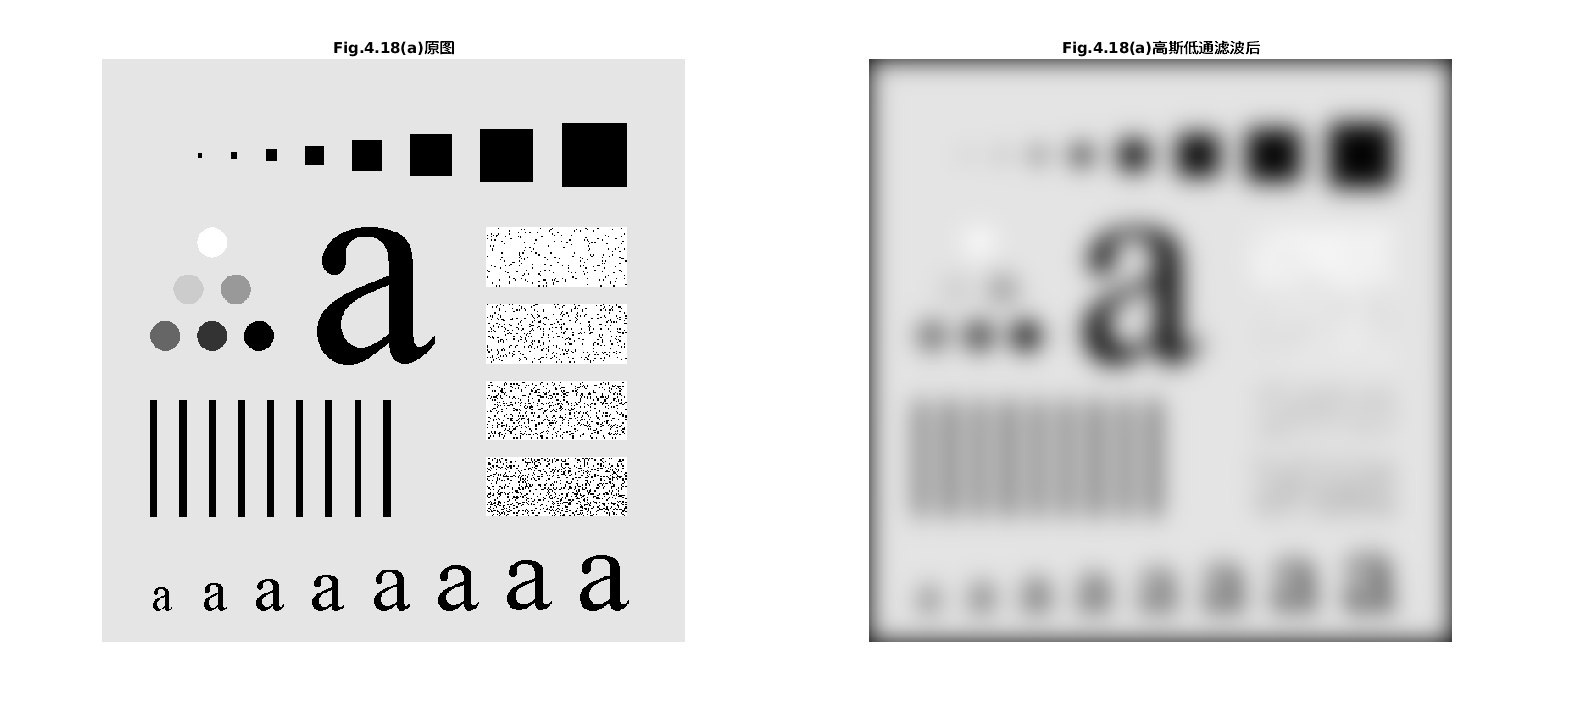
\includegraphics[width=0.8\linewidth]{fig/02.png}
\end{figure}


\section{高通滤波器(PROJECT 04-04)}
% PROJECT 04-04 Highpass Filtering Using a Lowpass Image
% (a) Subtract your image in Project 04-03(b) from the original to obtain a sharpened image, as in Eq. (4.4-14). You will note that the resulting image does not resemble the Gaussian highpass results in Fig. 4.26. Explain why this is so.
% (b) Adjust the variance of your Gaussian lowpass filter until the result obtained by image subtraction looks similar to Fig. 4.26(c). Explain your result.
\subsection{原理}
利用下式可以得到高通滤波的图像
\[f_{hp}(x,y)=f(x,y)-f_{lp}(x,y)\]
其中$f_{lp}$即为PROJECT 04-04通过高斯滤波后的图像。

\subsection{实验结果与分析}
用原图像减去高斯低通滤波后图像的方法得到的高通图像与直接进行高斯高通滤波的方法产生的图像没有太大区别,事实上
\[F(u,v)-F(u,v)H(u,v)=F(u,v)(1-H(u,v))=F(u,v)G(u,v)\]
其中$H$为高斯低通滤波器,$G$为高斯高通滤波器,因此这两种方式是等价的。
故存在差异的原因是数值计算的误差,即进行傅里叶变换时产生的数值差异导致两幅图像的差异。
\begin{figure}[H]
\centering
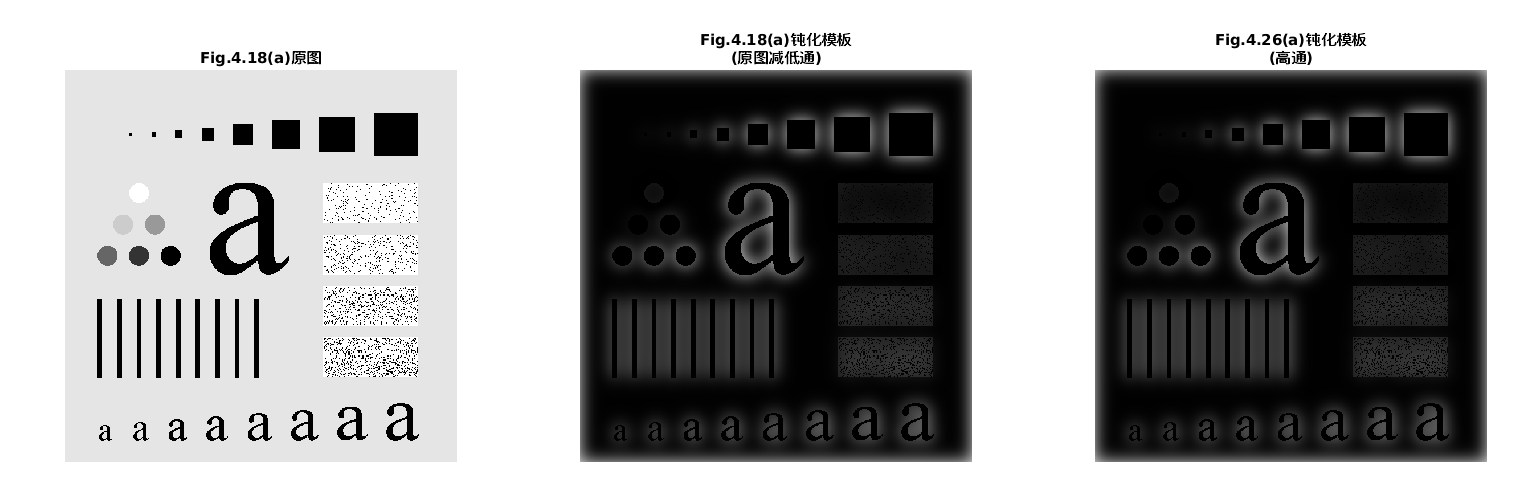
\includegraphics[width=0.8\linewidth]{fig/03.png}
\end{figure}

通过加大$\sigma$的值,可以使高斯低通滤波器作用的范围更大,进而剩余的高通分量更少,也即图像只剩部分细节可见。
可以看到下图已经和图4.26(c)非常接近了,这里选择的$\sigma=80$。
\begin{figure}[H]
\centering
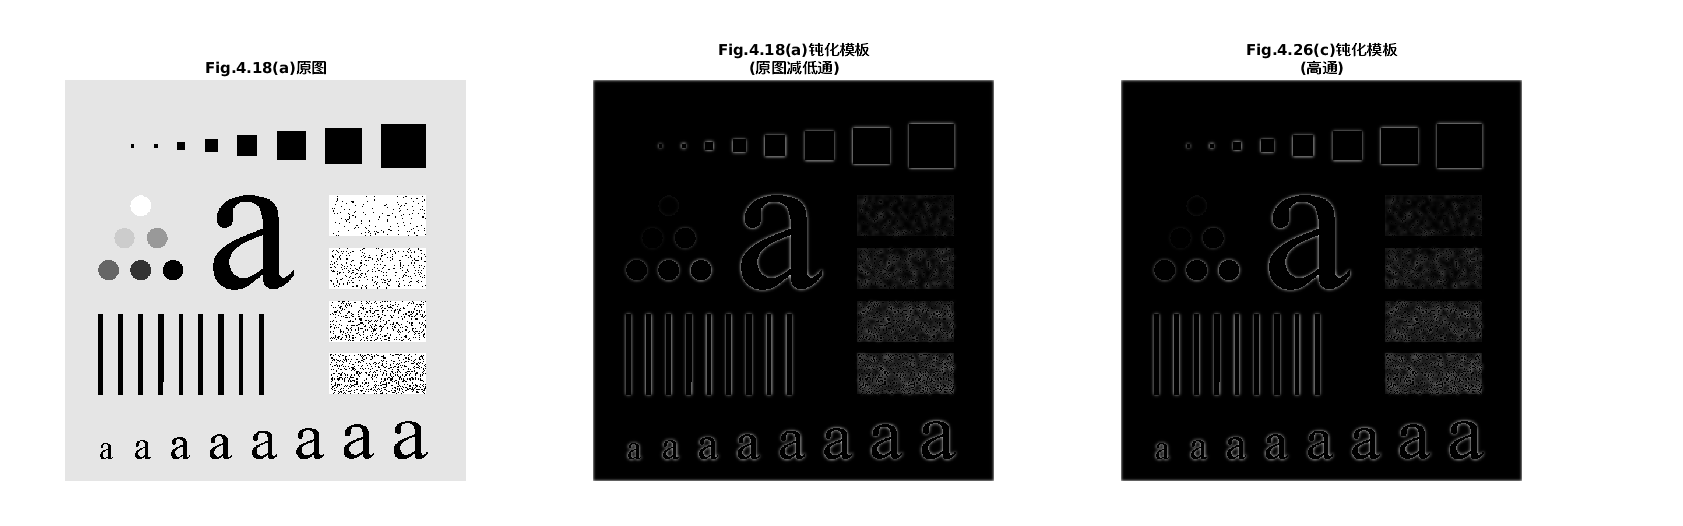
\includegraphics[width=0.9\linewidth]{fig/04.png}
\end{figure}

\section{频率域的相关(PROJECT 04-05)}
% PROJECT 04-05
% Correlation in the Frequency Domain Download Figs. 4.41(a) and (b) and duplicate Example 4.11 to obtain Fig. 4.41(e). Give the (x,y) coordinates of the location of the maximum value in the 2D correlation function. There is no need to plot the profile in Fig. 4.41(f).
\subsection{原理}
利用空间域的相关与频率域的乘积构成傅里叶变换对这一性质
\[f(x,y)\circ h(x,y)\iff F^\star(u,v)H(u,v)\]

\subsection{实验结果与分析}
相关性结果如下图所示。
若$f$为原图,$g$为掩膜/需要查找的图像,并且延拓后的图像大小为$M\times N$,要查找的图像在原图左上角$(x_0,y_0)$的位置,则两图计算出相关性系数的最大值的位置为$(M-x_0,N-y_0)$。
\begin{figure}[H]
\centering
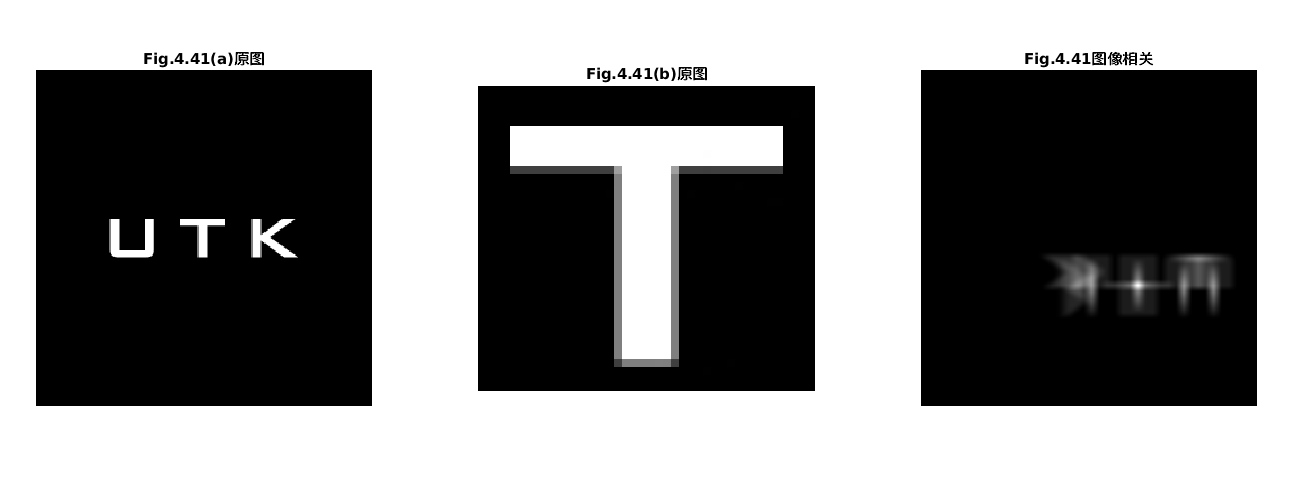
\includegraphics[width=\linewidth]{fig/05.png}
\end{figure}

通过Matlab计算可以找出最大值出现在$(191,193)$的位置,符合上述结论。

\section{傅里叶变换的旋转性质}
% 以Fig4.4为例检验谱平面随着图像旋转而旋转的性质。
\subsection{原理}
引入极坐标
\[x=r\cos\theta,y=r\sin\theta,u=\omega\cos\phi,v=\omega\sin\phi\]
有
\[f(r,\theta+\theta_0)\iff F(\omega,\phi+\theta_0)\]

\subsection{实验结果与分析}
从下图可以看出,当原图进行旋转时,频域确实也以相同的角度和方向旋转。
\begin{figure}[H]
\centering
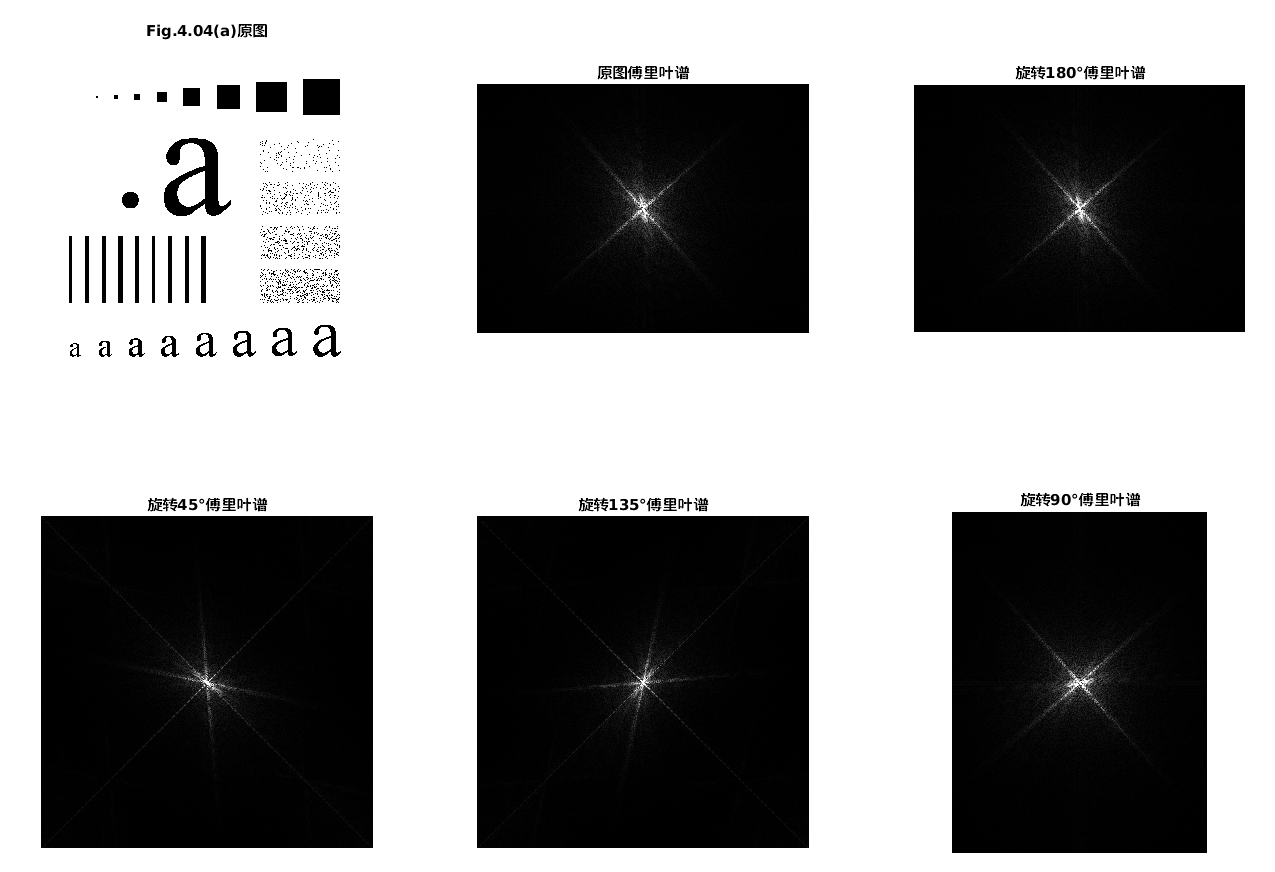
\includegraphics[width=\linewidth]{fig/06.png}
\end{figure}


\appendix\appendixconfig
\section{完整PROJECT代码}
\begin{lstlisting}
close all;clear all;clc;

% PROJECT 04-02
% (a)
I = imread('Fig0418(a).tif');
I = double(I);
[m,n] = size(I);
fftI = fft2(centerize(I));
sp = spectrum(fftI);

% (b)
figure,
subplot(121),imshow(uint8(I));
title('Fig.4.18(a)`原图'')
subplot(122),imshow(uint8(sp.^0.4),[]); % (log(1 + sp),[]);
title('Fig.4.18(a)`傅里叶谱'')

% (c)
s = sum(sum(I));
avg = s / (m * n)
fftOrig = fft2(I);
avg_fourier = fftOrig(1,1) / (m*n)

% PROJECT 04-03 (b)
gimg = gauss_lowpass(I,m/2,n/2,15);
figure,
subplot(121),imshow(uint8(I));
title('Fig.4.18(a)`原图'')
subplot(122),imshow(uint8(gimg));
title('Fig.4.18(a)`高斯低通滤波后'')

% PROJECT 04-04
% (a)
simg = I - gimg;
simg1 = gauss(I,15,0);
figure,
subplot(131),imshow(uint8(I));
title('Fig.4.18(a)`原图'')
subplot(132),imshow(uint8(simg));
title({'Fig.4.18(a)`钝化模板'';'(`原图减低通')'})
subplot(133),imshow(uint8(simg1));
title({'Fig.4.26(a)`钝化模板'';'(`高通')'})

% (b)
simg2 = I - gauss(I,80,1);
simg22 = gauss(I,80,0);
figure,
subplot(131),imshow(uint8(I));
title('Fig.4.18(a)`原图'')
subplot(132),imshow(uint8(simg2));
title({'Fig.4.18(a)`钝化模板'';'(`原图减低通')'})
subplot(133),imshow(uint8(simg22));
title({'Fig.4.26(c)`钝化模板'';'(`高通')'})

% PROJECT 04-05
I1 = imread('Fig0441(a).png');
I2 = imread('Fig0441(b).png');
[m1,n1] = size(I1);
[m2,n2] = size(I2);
P = 298;
Q = 298;
img1 = zeros(P,Q);
img2 = zeros(P,Q);
img1(1:m1,1:n1) = I1(1:m1,1:n1);
img2(1:m2,1:n2) = I2(1:m2,1:n2);
cimg1 = centerize(img1);
cimg2 = centerize(img2);
f1 = fft2(cimg1);
f2 = fft2(cimg2);
% rel = conj(f1).* f2;
rel = f2 .* conj(f1);
newI = recover(ifft2(rel));
figure,
subplot(131),imshow(uint8(I1));
title('Fig.4.41(a)`原图'')
subplot(132),imshow(uint8(I2));
title('Fig.4.41(b)`原图'')
subplot(133),imshow(uint8(newI.^0.3));
title('Fig.4.41`图像相关'')
max_value = max(max(newI));
[row,col] = find(newI == max_value)

% Fig 4.04(a)
Ir = imread('Fig0404(a).png');
I0 = frotate(Ir,0);
I1 = frotate(Ir,45);
I2 = frotate(Ir,90);
I3 = frotate(Ir,135);
I4 = frotate(Ir,180);
figure,
subplot(231),imshow(I);
title('Fig.4.04(a)`原图'')
subplot(232),imshow(log(I0 +1));
title('`原图傅里叶谱'')
subplot(233),imshow(log(I4 +1));
title('`旋转180$\degree$傅里叶谱'')
subplot(234),imshow(log(I1 +1));
title('`旋转45$\degree$傅里叶谱'')
subplot(235),imshow(log(I3 +1));
title('`旋转135$\degree$傅里叶谱'')
subplot(236),imshow(log(I2 +1));
title('`旋转90$\degree$傅里叶谱'')

% PROJECT 04-03 (a)
function g = gauss(img,sig,lowpass_flag)
	[M,N] = size(img);
	P = 2 * M; Q = 2 * N; % remember to do extension
	Iext = zeros(P,Q);
	Iext(1:M,1:N) = img(1:M,1:N);
	[Y,X] = meshgrid(1:Q,1:P);
    center_x = P/2; center_y = Q/2;
	D = (X - center_x).^2 + (Y - center_y).^2;
	if lowpass_flag == 1
		H = exp(-D/(2*sig^2));
	else
		H = 1 - exp(-D/(2*sig^2));
    end
	cimg = centerize(Iext);
	f = fft2(cimg);
	g = centerize(real(ifft2(H.*f)));
	g = g(1:M,1:N);
end

% PROJECT 04-01
% (a)
function g = centerize(img)
	[M,N] = size(img);
	[Y,X] = meshgrid(1:N,1:M);
	ones = (-1).^(X+Y);
	g = ones.*img;
end

% (b)
function g = mul_real(A,c)
	% g = c * real(A) + c * imag(A) * i;
	g = c * A;
end

% (c)
function g = inverse_fft(A)
	g = ifft2(A);
end

% (d)
function g = recover(A)
	g = centerize(real(A));
end

% (e)
function g = spectrum(A)
	g = abs(A);
end

% rotate
function g = frotate(img,ang)
	rI = imrotate(img,ang);
	FI = ifft2(centerize(double(rI)));
	g = abs(FI);
end
\end{lstlisting}

\end{document}

% Suggested Format for Submitting Project Reports
% Because laboratory projects are in addition to course work, it is suggested that project
% reports be kept short, and be organized in a uniform manner to simplify grading. The
% following format achieves these objectives.

% Page 1. Cover Page. Typed or printed neatly.
% · Project title
% · Project number
% · Course number
% · Student's name
% · Date due
% · Date handed in
% · Abstract (not to exceed 1/2 page)

% Page 2. Technical discussion. One to two pages (max). This section should include the
% techniques used and the principal equations (if any) implemented.

% Page 3 (or 4). Discussion of results. One to two pages (max). A discussion of results
% should include major findings in terms of the project objectives, and make clear
% reference to any images generated.

% Results. Includes all the images generated in the project. Number images individually
% so they can be referenced in the preceding discussions.

% Appendix. Program listings. Includes listings of all programs written by the student.
% Standard routines and other material obtained from other sources should be
% acknowledged by name, but their listings should not be included.

% Layout. The entire report must be in standard sheet size format (8.5 x 11 inches in the
% U.S.) All sheets should be stapled in three locations to form a binding booklet-like
% support on the left margin. Alternatively, sheets can be assembled using a commercial
% plastic binding product with a clear plastic cover.

% A note on program implementation: As noted earlier, the objective of the computer
% programs used in the following projects is to teach the student how to manipulate
% images. There are numerous packages that perform some of the functions required to
% implement the projects. However, the use of "canned" routines as the only method to
% implement an entire project is discouraged. For example, if the students are using
% MATLAB and the Image Processing Toolbox, a balanced approach is to use MATLAB's
% programming environment to write M functions to implement the projects, using some of
% MATLAB's own functions in the process. A good example is the implementation of the 2-
% D Fourier Fast Transform. The student should use the MATLAB function that computes
% the 2-D FFT directly, but write functions for operations such as centering the transform,
% multiplying it by a filter function, and obtaining the spectrum.